%!TEX root = main.tex
\section{Background}
This section provide technical details about the four main serverless providers, namely Amazon Web Services (\S\ref{sec:ss:aws}), Microsoft Azure (\S\ref{sec:ss:azure}), Google Cloud (\S\ref{sec:ss:google}) and IBM Cloud (\S\ref{sec:ss:ibm}). 
\vs{MAISSEN that the next sentence is true:} We compare the performance of all of them in our evaluation (see Section~\ref{sec:evaluation}).

%In this chapter, the choice of serverless computing providers and the choice of runtimes respectively programming languages is derived. Furthermore, the implemented tests will be explained in detail and it is shown what their effect and importance is.

%\subsection{Choosing Serverless Computing Providers}
%\label{sec:CSP}
%
%There are a lot of cloud providers available and many of them are trying to grow and therefore investing more and more in their infrastructure. So this benchmark suite could have taken into account as many cloud providers as possible, assumed they provide serverless computing, but that would have exceeded the scope of this thesis. Figure \ref{fig:market_share} illustrates on the left hand side the global revenue of the cloud infrastructure services market which has reached nearly \$23 billion in the second quarter of 2019. What's more interesting for choosing cloud providers for this benchmark suite is the market share. As one can see in figure \ref{fig:market_share} on the right hand side the market share of cloud computing is mainly dominated by a few big players: Amazon, Microsoft, Google, \gls{IBM} and Alibaba. Amazon still is the unprecedented leader in this field of business. Nevertheless, other competitors are heavily investing in the cloud business. Google will invest 3 billion euros in its European data centers as Sundar Pichai, the \gls{CEO} of Google, stated in the Google blog \cite{GoogleBlog}. And also Microsoft has recently been given a \$10 billion contract by the US Department of Defense to transform the military's cloud computing systems \cite{NYJEDI, JEDI}.
%
%\begin{figure}[htp]
%\begin{center}
%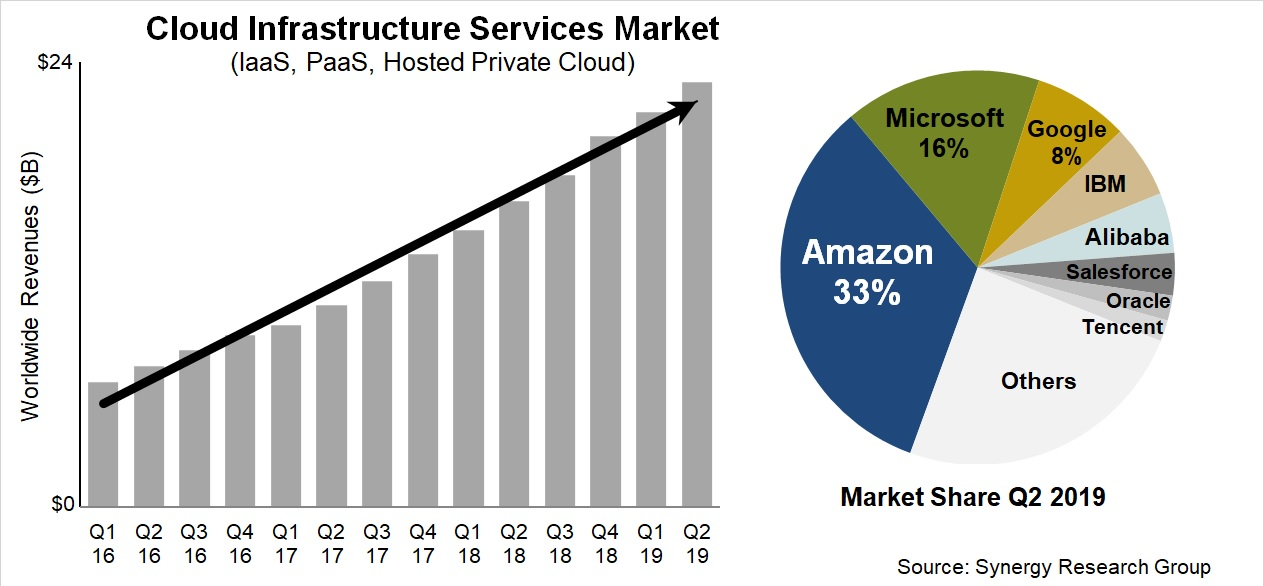
\includegraphics[width=0.5\textwidth]{bilder/synergy.jpg}
%\captionsetup[table]{justification=centering, labelfont=bf}
%\caption[Cloud Infrastructure Services Market Share]{Cloud Infrastructure Services Market Share\\Source: Synergy Research Group \cite{Synergy}}
%\label{fig:market_share}
%\end{center}
%\end{figure}
%
%For the above mentioned reasons, the following top four providers were taken into consideration.
%\begin{itemize}
%  \item Amazon Web Services
%  \item Microsoft Azure
%  \item Google Cloud
%  \item IBM Cloud
%\end{itemize}
%All of them offer a serverless platform which will be described for each cloud provider in the following sections.

%\begin{remark}
%At the beginning of this thesis, a deployment on Apache OpenWhisk was considered on the private cluster of the university of Neuchâtel. After several time wasting and failed attempts to set up OpenWhisk and contradicting documentation on the OpenWhisk website respectively the GitHub page of OpenWhisk the idea was dropped. Since \gls{IBM} uses an implementation based on OpenWhisk, the performance is expected to be similar. Nevertheless, it would have been interesting to compare those two very similar or even identical systems on a private and on a public cloud.
%\end{remark}

\subsection{Amazon Web Services Lambda}\label{sec:ss:aws}

\gls{AWS} Lambda~\cite{AWSLambda} was released in November in 2014 \cite{AWSLambdaRelease}. 
\gls{AWS} Lambda spans 18 geographically dispersed regions, plus China\cite{AWSRegions}. 
At the time of writing, it supports six different runtimes and seven different programming languages \cite{AWSLambdaLanguages}. 
Depending on the region where the function is deployed, Lambda supports up to 3000 instances to serve the user' functions~\cite{AWSLambdaScaling}. 
The memory allocated to a function instance can vary from 128 \gls{MB} up to 3008 \gls{MB} in steps of 64 \gls{MB}~\cite{AWSLambdaConfig}. 
The \gls{CPU} power increases linearly with its memory allocation.
Forinstance, at 1792 \gls{MB} the function will get 1 \gls{vCPU}~\cite{AWSLambdaConfig}.\vs{MAISSEN: why 1792?}

As observed in~\cite{216063}, Lambda executes functions using two different \gls{CPU}s, namely Intel Xeon E5-2666 clocked at 2.90 \gls{GHz}  and the Intel Xeon E5-2680, clocked at 2.80 \gls{GHz} respectively. 
%This information was extracted by Wang et al. from the file \texttt{/proc/cpuinfo} in the Linux operating system.
%\begin{remark} From my own experience I can tell that cloud providers generally don't like to tell their customers every detail of hardware they use or how exactly services are implemented. The first point might be true because they don't want to tell a customer what exact \gls{CPU}s he gets, because then he will certainly complain if it differs from the specification and the provider has to take responsibility. The second point should be obvious for economic and competition related reasons.
%\end{remark}
%Knowing that, one can more or less estimate the theoretical computing power that the virtual \gls{CPU} will provide. 
%\begin{remark}
%The pricing of \gls{AWS} Lambda and all the other services will be discussed in section \ref{sec:pricing} Pricing.
%\end{remark}

\subsection{Microsoft Azure Functions}\label{sec:ss:azure}

Microsoft Azure Functions~\cite{AzureFunctions} was released publicly in Novenber 2016~\cite{AzureFunctionsAnnouncement}. %in preview (Microsoft's term for beta) and then later in November 2016 it became generally available \cite{AzureFunctionsAnnouncement}. 
it supports five runtimes and seven different programming languages~\cite{AzureFunctionsLanguages}.
Compared to the other three cloud providers, Azure offers three different hosting plans \cite{AzureFunctionsPlans}:
%Something a little different with Azure compared to the other three cloud providers is that one can select between three different hosting plans \cite{AzureFunctionsPlans}:
Azure Functions offers billing plans that adapt to the load and popularity of the deployed function (\emph{e.g.}, the consumption plan), plans with finer-grain control over the computing instance size and pre-warming support (\emph{e.g.}, a premium plan), and an billing plan customized on a given application needs (\emph{e.g.}, the app service plan). 
This work only considers the consumption plan (generation 2.0~\cite{AzureFunctionsGenerations}), being the only one to be fully managed by the cloud provider and the most similar in the features to the ones offered by the alternative provders. 
%\begin{itemize}
%\item[] \textbf{Consumption plan:} It adds and removes instances dynamically depending on the load on the function and cost only arise when functions are running. This is the most 'serverless' option among those three.
%\item[] \textbf{Premium plan:} The premium plan is similar to the consumption plan but offers more integration and control over the functions. Instance sizes can be chosen and instances can be pre-warmed. The cost is calculated with \gls{CPU} and \gls{GB} memory used per second.
%\item[] \textbf{App Service plan:} How many and on which \gls{VM}s the functions run can be decided in the App Service plan. Scaling happens manually, time based or based on metrics such as \gls{CPU} usage.
%\end{itemize}
%This thesis will only consider the consumption plan, as it is the default plan and fully managed, and therefore \textit{more} serverless than the others. Additionally, it is similar to the services of the other providers.\\
%There are currently three different generations of the service available \cite{AzureFunctionsGenerations}, this project uses generation 2.

Azure Functions can use as many as 200 instances and up to 1.5GB memory~\cite{AzureFunctionsPlans}. 
The service can run either on Windows or Linux hosts, and is offered in 28 out of 46 publicly accessible regions~\cite{AzureRegions}.
Note that the consumption plan is only available in 11 regions for both Linux and Windows, hence we restrict to those in our experiments.
Computing nodes can be characterized by their \gls{ACU}, with 100 ACU roughly map to 1 \gls{vCPU}.
%For computing power, Azure has its own term named \gls{ACU} index, where 100 ACU roughly map to 1 \gls{vCPU}.
%The instances in the Azure functions consumption plan have an \gls{ACU} of 100 which is about the equivalent of 1 \gls{vCPU}. 
According to our investigations, we believe Azure Functions to be executed by virtual machiens of type \textit{Av2}\vs{MAISSEN: which ones from \url{https://aws.amazon.com/ec2/instance-types/}? Clarify.}, as it most closely resembles its declared \gls{ACU}~\cite{AzureFunctionsVMs}. 
These \gls{VM}s use three different \gls{CPU}s: Intel Xeon 8171M at 2.1 \gls{GHz}, Intel Xeon E5-2673 v4 at 2.3 \gls{GHz} and Intel Xeon E5-2673 v3 at 2.4 \gls{GHz}~\cite{AzureFunctionsVMs}.

\subsection{Google Cloud Functions}\label{sec:ss:google}
%\vs{STOPPED HERE}
%On the Google Cloud Platform, the serverless service is simply called \textit{Functions} \cite{GoogleFunctions}. 
Google Functions~\cite{GoogleFunctions} was released on July in 2018~\cite{GoogleFunctionsReleases}, and currently available through seven out of twenty regions~\cite{GoogleFunctionsLocations}.
%Compared to AWS and Azure that is two and a half years respectively one year later for the first release. 
It currently only supports three programming languages~\cite{GoogleFunctionsLanguages}, namely \vs{MAISSEN: FIX}. 
While there is not a maximum number of allocated instances per single function, it only allows up to 1000 functions to be executed concurrently~\cite{GoogleFunctionsQuotas}.
%The documentation does not mention a limit of maximum allocated instances per function. 
%However, it states that at maximum 1000 functions can be concurrently in execution \cite{GoogleFunctionsQuotas}.
Table~\ref{table:google_functions_cpu_ram} summarizes the options for CPU and memory combinations supported by the platform\cite{GoogleFunctionsPricing}.
While the official \emph{Functions} documentation lacks details on the exact CPU models, a quick inspection of \texttt{/proc/cpuinfo} unveils certain details, such as \texttt{vendor\_id}, \texttt{cpu\_family} and \texttt{model}.
We report on the use of Intel-based processors as well as some specific generation details in \vs{MAISSEN: FIX where?}.
%Possible options for CPU and memory allocation per instance are shown in table \ref{table:google_functions_cpu_ram} \cite{GoogleFunctionsPricing}. 
%The service is available in seven out of twenty regions~\cite{GoogleFunctionsLocations}.

\begin{table}[!t]

\caption[Google Cloud Functions - Possible memory allocation and corresponding CPU frequency]{Google Cloud Functions - Possible memory allocation and corresponding CPU frequency~\cite{GoogleFunctionsPricing}.}
%\captionsetup[table]{justification=centering, labelfont=bf}
\centering
\resizebox{\columnwidth}{!}{
\begin{tabular}{l|r|r|r|r|r} 
 \hline
	\textbf{Memory} & 128\gls{MB} & 256\gls{MB} & 512\gls{MB} & 1024\gls{MB} & 2048\gls{MB} \\ 
	\textbf{CPU} & 200\gls{MHz} & 400\gls{MHz} & 800\gls{MHz} & 1.4 \gls{GHz} & 2.4 \gls{GHz} \\
	\hline
\end{tabular}
\vspace{-10pt}
}
\label{table:google_functions_cpu_ram}
\end{table}

%Google does not mention what type of CPU they use for functions on the underlying infrastructure. 
%The CPU type could also not be extracted by Wang et al. \cite{216063} and the file \texttt{/proc/cpuinfo} does not show information on the CPU model name. 
%It shows however information for the fields \texttt{vendor\_id}, \texttt{cpu\_family} and \texttt{model}. 
%Those values reveal that Intel processors are used and can give an indication from which generation the CPU is. 
%\vs{See the example file content \ref{lst:cpuinfo} in the appendix.} 

\subsection{IBM Cloud Functions}\label{sec:ss:ibm}

\gls{IBM}'s Cloud Functions \cite{IBMFunctions} is built atop Apache OpenWhisk, an open source serverless cloud platform using Docker containers~\cite{OpenWhisk}. 
As such, in addition to Docker, it supports eight additional runtimes~\cite{IBMRuntimes}, such as \vs{MAISSEN: list them all here}.
%\gls{IBM} Cloud Functions supports nine different runtimes including a Docker runtime \cite{IBMRuntimes}. 
The service is restricted to 1000 concurrently active executions (including those enqueued for execution) per namespace~\cite{IBMLimits}. 
%However this limit can be increased for a specific business case but needs to be applied for via the ticketing system of the \gls{IBM} support \cite{IBMLimits}. 
Memory allocation can be set from 128 \gls{MB} to 2048 \gls{MB} in steps of 32 \gls{MB}. 
\gls{IBM} Cloud Functions is available in five out of six regions \cite{IBMLocations}.\footnote{One region\vs{MAISSEN: which one?} lacks support for Cloud Foundry~\cite{IBMCloudFoundry} and as such it not be used to deply via the \gls{CLI}, and hence it is not included in this work.} 
%The documentation does not mention anything on \gls{CPU} or machines they are using. 
Our experiments revelaed that some of the  instances supporting the execution of the functions run on top of Intel Xeon E5-2683 v3 at 2.00 \gls{GHz}.
\vs{See the example file content \ref{lst:cpuinfo2} in the appendix.}



